\section{A Semantic Wiki for e-Science}

\begin{wrapfigure}{r}{5.5cm}
  \centering
  \vspace{-.5cm}
  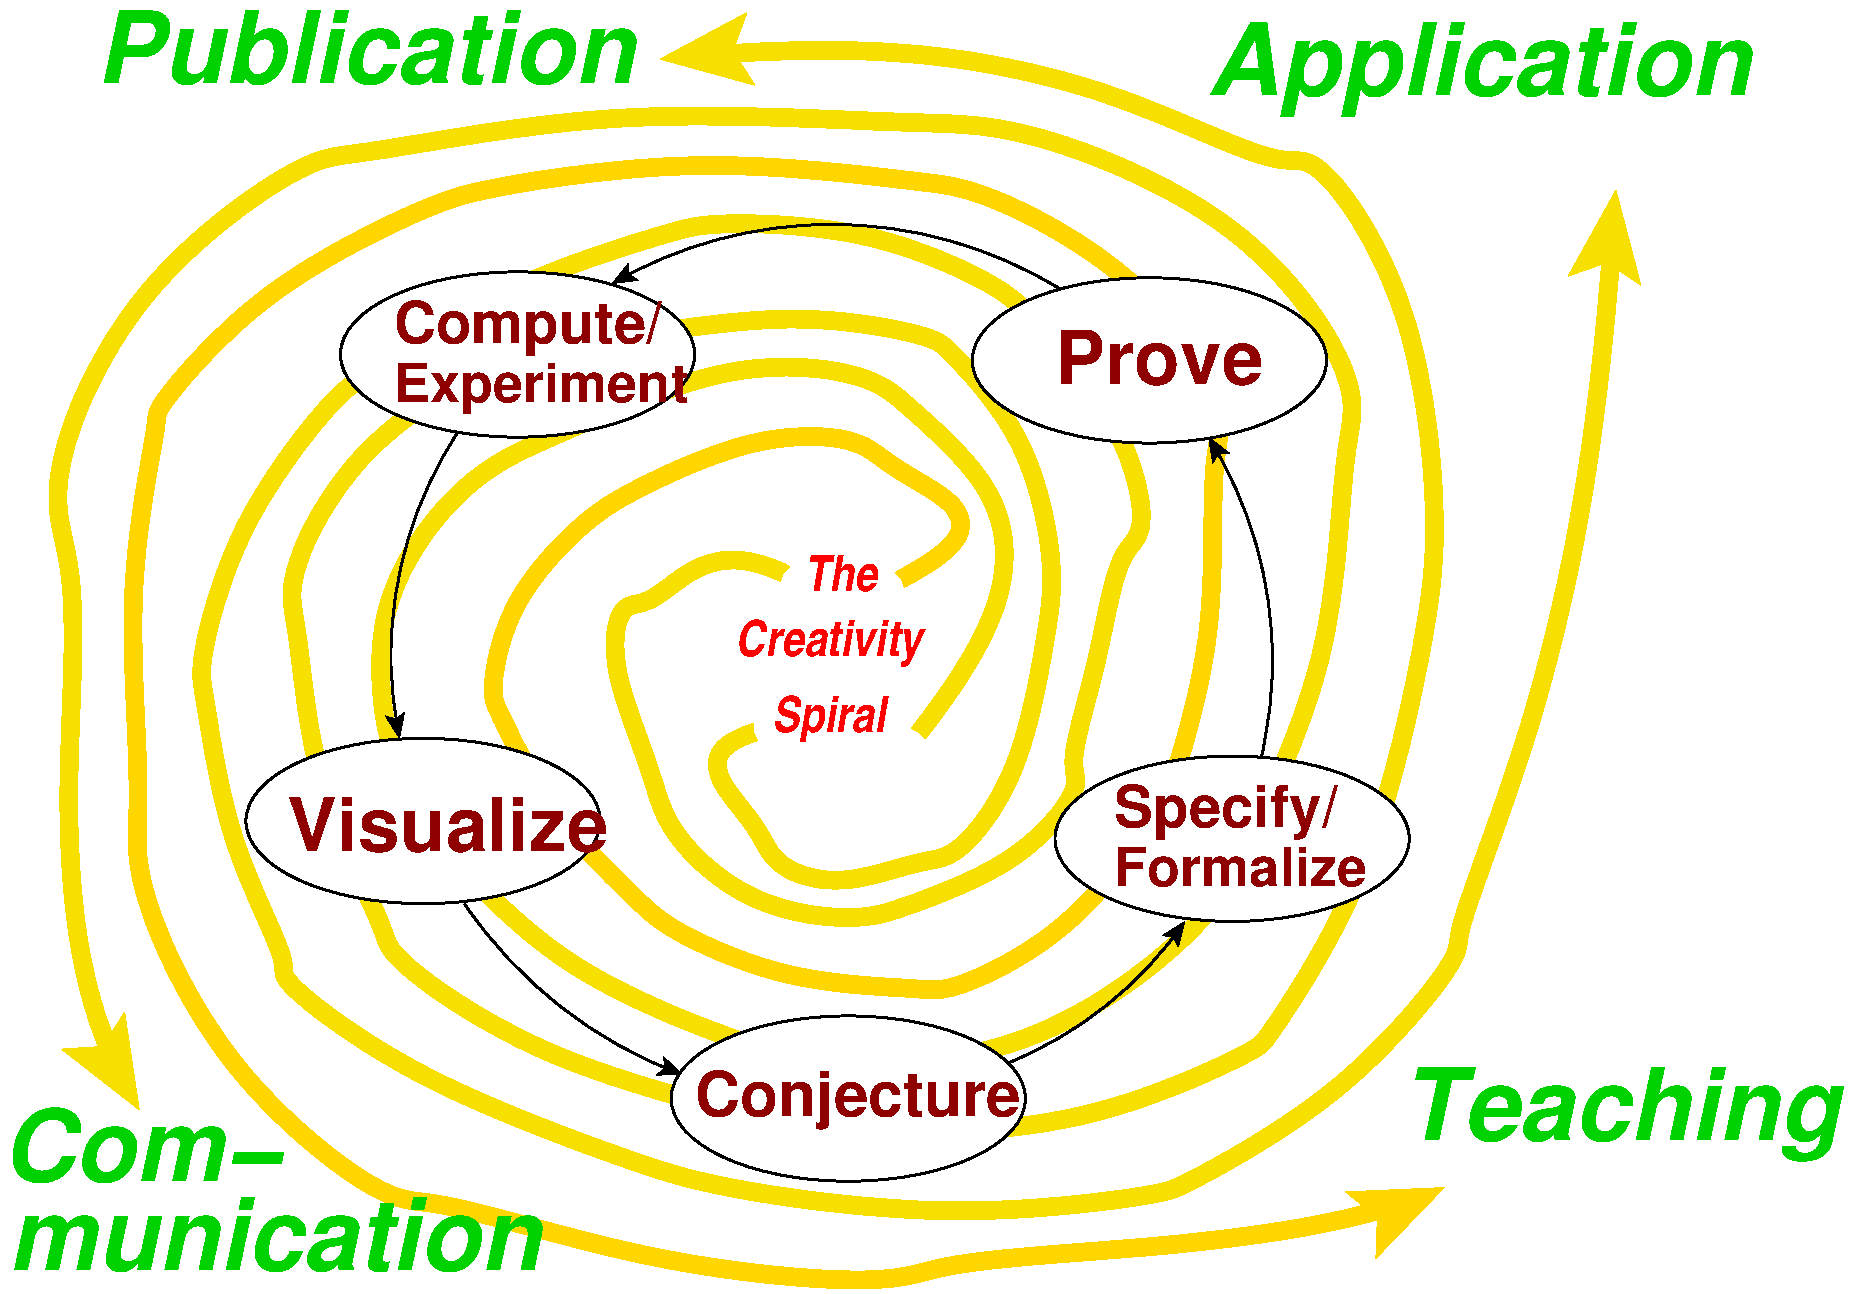
\includegraphics[width=5cm]{creativity-spiral}
  \vspace{-.5cm}
  \caption{The Math/Science Creativity Spiral (after Buchberger, 1995)}
  \label{fig:creativity-spiral}
\end{wrapfigure}

\ednote{@Sean:  Why do you start off talking about authoring documents?  What we are doing
(in theory) is much more than this.  It is nothing less than managing the entire Flyspeck
project, what could be an essential part of completing the task, not simply
writing about it.  I think this section should be more lofty.}

A great deal of scientific work consists of collaboratively authoring documents --- taking
down first hypotheses, commenting on results of experiments or project steps, as well as
structuring, annotating, and re-organizing existing items of knowledge.  Tools
that \emph{understand} the knowledge contained in scientific documents are desirable for
editing such documents.  One approach towards this is writing scientific documents in a semantic
markup language with an editor that knows the structures available in this language.

Besides generic approaches like SALT~\cite{Groza:SALT07}, semantic markup has been most
deeply investigated in the specific domain of mathematics with its complex and explicit
structures\ednote{reword}, resulting in languages like MathML, OpenMath, \ednote{references} and
OMDoc~\cite{Kohlhase:omdoc1.2}.  OMDoc is a language that employs Content
MathML\footnote{MathML comes in two flavors: Presentation MathML expresses the way a
  formula is rendered, whereas Content MathML models its logical structure.  Formal
  mathematical software like a Computer Algebra System would export formulae in Content
  MathML, but for publishing, they would be converted to Presentation MathML.} or OpenMath
for structurally representing mathematical \emph{objects} (symbols, numbers, equations,
etc.) and adds two layers on top of that: Objects or informal text can be annotated as
mathematical \emph{statements} (symbol declarations, definitions, axioms, theorems,
proofs, examples, etc.), and collections of interrelated statements are grouped into
\emph{theories}.

With SWiM, a semantic wiki for mathematical knowledge management (see
section~\ref{sec:swim}), we have investigated collaborative editing of OMDoc documents.  It
has turned out that a wiki is a suitable tool for supporting the incremental workflow of
scientific writing.  But wikis have not only shown to be appropriate for \emph{writing},
but also for project management, e.\,g.\ in corporate settings~\cite{leuf01:wikiway}.
Thus, we are interested in applying our technologies to scientific knowledge engineering
projects.  The Flyspeck project (see section~\ref{sec:flyspeck}) was particularly
appealing as a use case: It involves both highly formal and semi-formal mathematical
knowledge, as well as informal text, and it was found \ednote{FR: Was it, or are we investigating whether it is?} to be suitable for ``crowdsourcing''
and supporting the project organization by social software.  This is suggested by its
large extent and the required manpower.  We anticipate that the three conditions for
successful peer production stated by Tapscott and Williams~\cite{wikinomics} will hold or
can be satisfied by software support: The object of production is information, which keeps
the cost of participation low, tasks (i.\,e.\ lemmas to be proven) can mostly be broken
down into small, independent pieces, and the cost of integrating the individual
contributions is low\ednote{FR: Should we discuss whether it is low?}.

